\documentclass[11pt,a4paper]{article}
\usepackage{amsmath}
\usepackage{amssymb}
\usepackage{booktabs}
\usepackage{longtable}
\usepackage{geometry}
\geometry{margin=1in}
\usepackage{hyperref}
\usepackage{enumitem}
\usepackage{graphicx}
\usepackage{siunitx}

\title{Engineering Calculation Report: Problem 2-2: Find Force with Known Resultant}
\date{October 13, 2025}

\begin{document}
\maketitle

\section*{Description}

    If the resultant force is to be 500 N directed along the positive y-axis,
    and F\textbackslash{}_2 = 700 N at 195°, determine the magnitude and direction of F\textbackslash{}_1.
    

\section{Known Variables}

\begin{longtable}{llSl}
\toprule
Symbol & Name & {Value} & Unit \\
\midrule
\endhead
$F_{1_mag}$ & F\textbackslash{}_1 Magnitude & 959.778 & N \\
$F_{1_angle}$ & F\textbackslash{}_1 Direction & 45.2121 & ° \\
$F_{2_mag}$ & F\textbackslash{}_2 Magnitude & 700 & N \\
$F_{2_angle}$ & F\textbackslash{}_2 Direction & -165 & ° \\
\bottomrule
\end{longtable}

\section{Unknown Variables (To Calculate)}

\begin{longtable}{lll}
\toprule
Symbol & Name & Unit \\
\midrule
\endhead
$F_{1_x}$ & F\textbackslash{}_1 X-Component & N \\
$F_{1_y}$ & F\textbackslash{}_1 Y-Component & N \\
$F_{2_x}$ & F\textbackslash{}_2 X-Component & N \\
$F_{2_y}$ & F\textbackslash{}_2 Y-Component & N \\
$F_{R_mag}$ & F\textbackslash{}_R Magnitude & N \\
$F_{R_angle}$ & F\textbackslash{}_R Direction & ° \\
$F_{R_x}$ & F\textbackslash{}_R X-Component & N \\
$F_{R_y}$ & F\textbackslash{}_R Y-Component & N \\
\bottomrule
\end{longtable}

\section{Equations Used}

\begin{enumerate}
\item $\Large F_{1}^{2} = F_{R}^{2} + F_{2}^{2} - 2 \cdot F_R \cdot F_2 \cdot \cos{gamma}$
\item $\Large \frac{\sin{alpha}}{F_2} = \frac{\sin{gamma}}{F_1}$
\end{enumerate}

\section{Step-by-Step Solution}

\begin{enumerate}[label=\textbf{Step \arabic*:},leftmargin=2cm]
\item \textbf{Solve for $F_{1 Magnitude}$}

\begin{description}[leftmargin=2cm]
\item[\textbf{Equation:}] \mbox{}

\begin{flalign*}
\Large F_{1}^{2} = F_{R}^{2} + F_{2}^{2} - 2 \cdot F_R \cdot F_2 \cdot \cos{gamma} &&
\end{flalign*}

\item[\textbf{Substitution:}] \mbox{}

\begin{flalign*}
\Large F_{1}^{2} = (500.00\,\text{N})^{2} + (700.00\,\text{N})^{2} - 2  \cdot  (500.00\,\text{N})  \cdot  (700.00\,\text{N})  \cdot  \cos{105.0^\circ} &&
\end{flalign*}

\item[\textbf{Result:}] \mbox{}

\begin{flalign*}
\Large F_{1 Magnitude} = 959.78\,N &&
\end{flalign*}

\end{description}

\item \textbf{Solve for $F_{1 Direction}$}

\begin{description}[leftmargin=2cm]
\item[\textbf{Equation:}] \mbox{}

\begin{flalign*}
\Large \frac{\sin{alpha}}{F_2} = \frac{\sin{gamma}}{F_1} &&
\end{flalign*}

\item[\textbf{Substitution:}] \mbox{}

\begin{flalign*}
\Large \frac{\sin{alpha}}{700.00\,\text{N}} = \frac{\sin{105.0^\circ}}{959.78\,\text{N}} &&
\end{flalign*}

\item[\textbf{Result:}] \mbox{}

\begin{flalign*}
\Large F_{1 Direction} = 45.21\,^\circ &&
\end{flalign*}

\end{description}

\end{enumerate}


\section{Summary of Results}

\begin{longtable}{llSl}
\toprule
Variable & Name & {Final Value} & Unit \\
\midrule
\endhead
$F_{1_x}$ & F\textbackslash{}_1 X-Component & 676.148 & N \\
$F_{1_y}$ & F\textbackslash{}_1 Y-Component & 681.173 & N \\
$F_{2_x}$ & F\textbackslash{}_2 X-Component & -676.148 & N \\
$F_{2_y}$ & F\textbackslash{}_2 Y-Component & -181.173 & N \\
$F_{R_mag}$ & F\textbackslash{}_R Magnitude & 500 & N \\
$F_{R_angle}$ & F\textbackslash{}_R Direction & 1.5708 & ° \\
$F_{R_x}$ & F\textbackslash{}_R X-Component & 3.06162e-14 & N \\
$F_{R_y}$ & F\textbackslash{}_R Y-Component & 500 & N \\
\bottomrule
\end{longtable}

\section{Vector Diagram}

\begin{center}
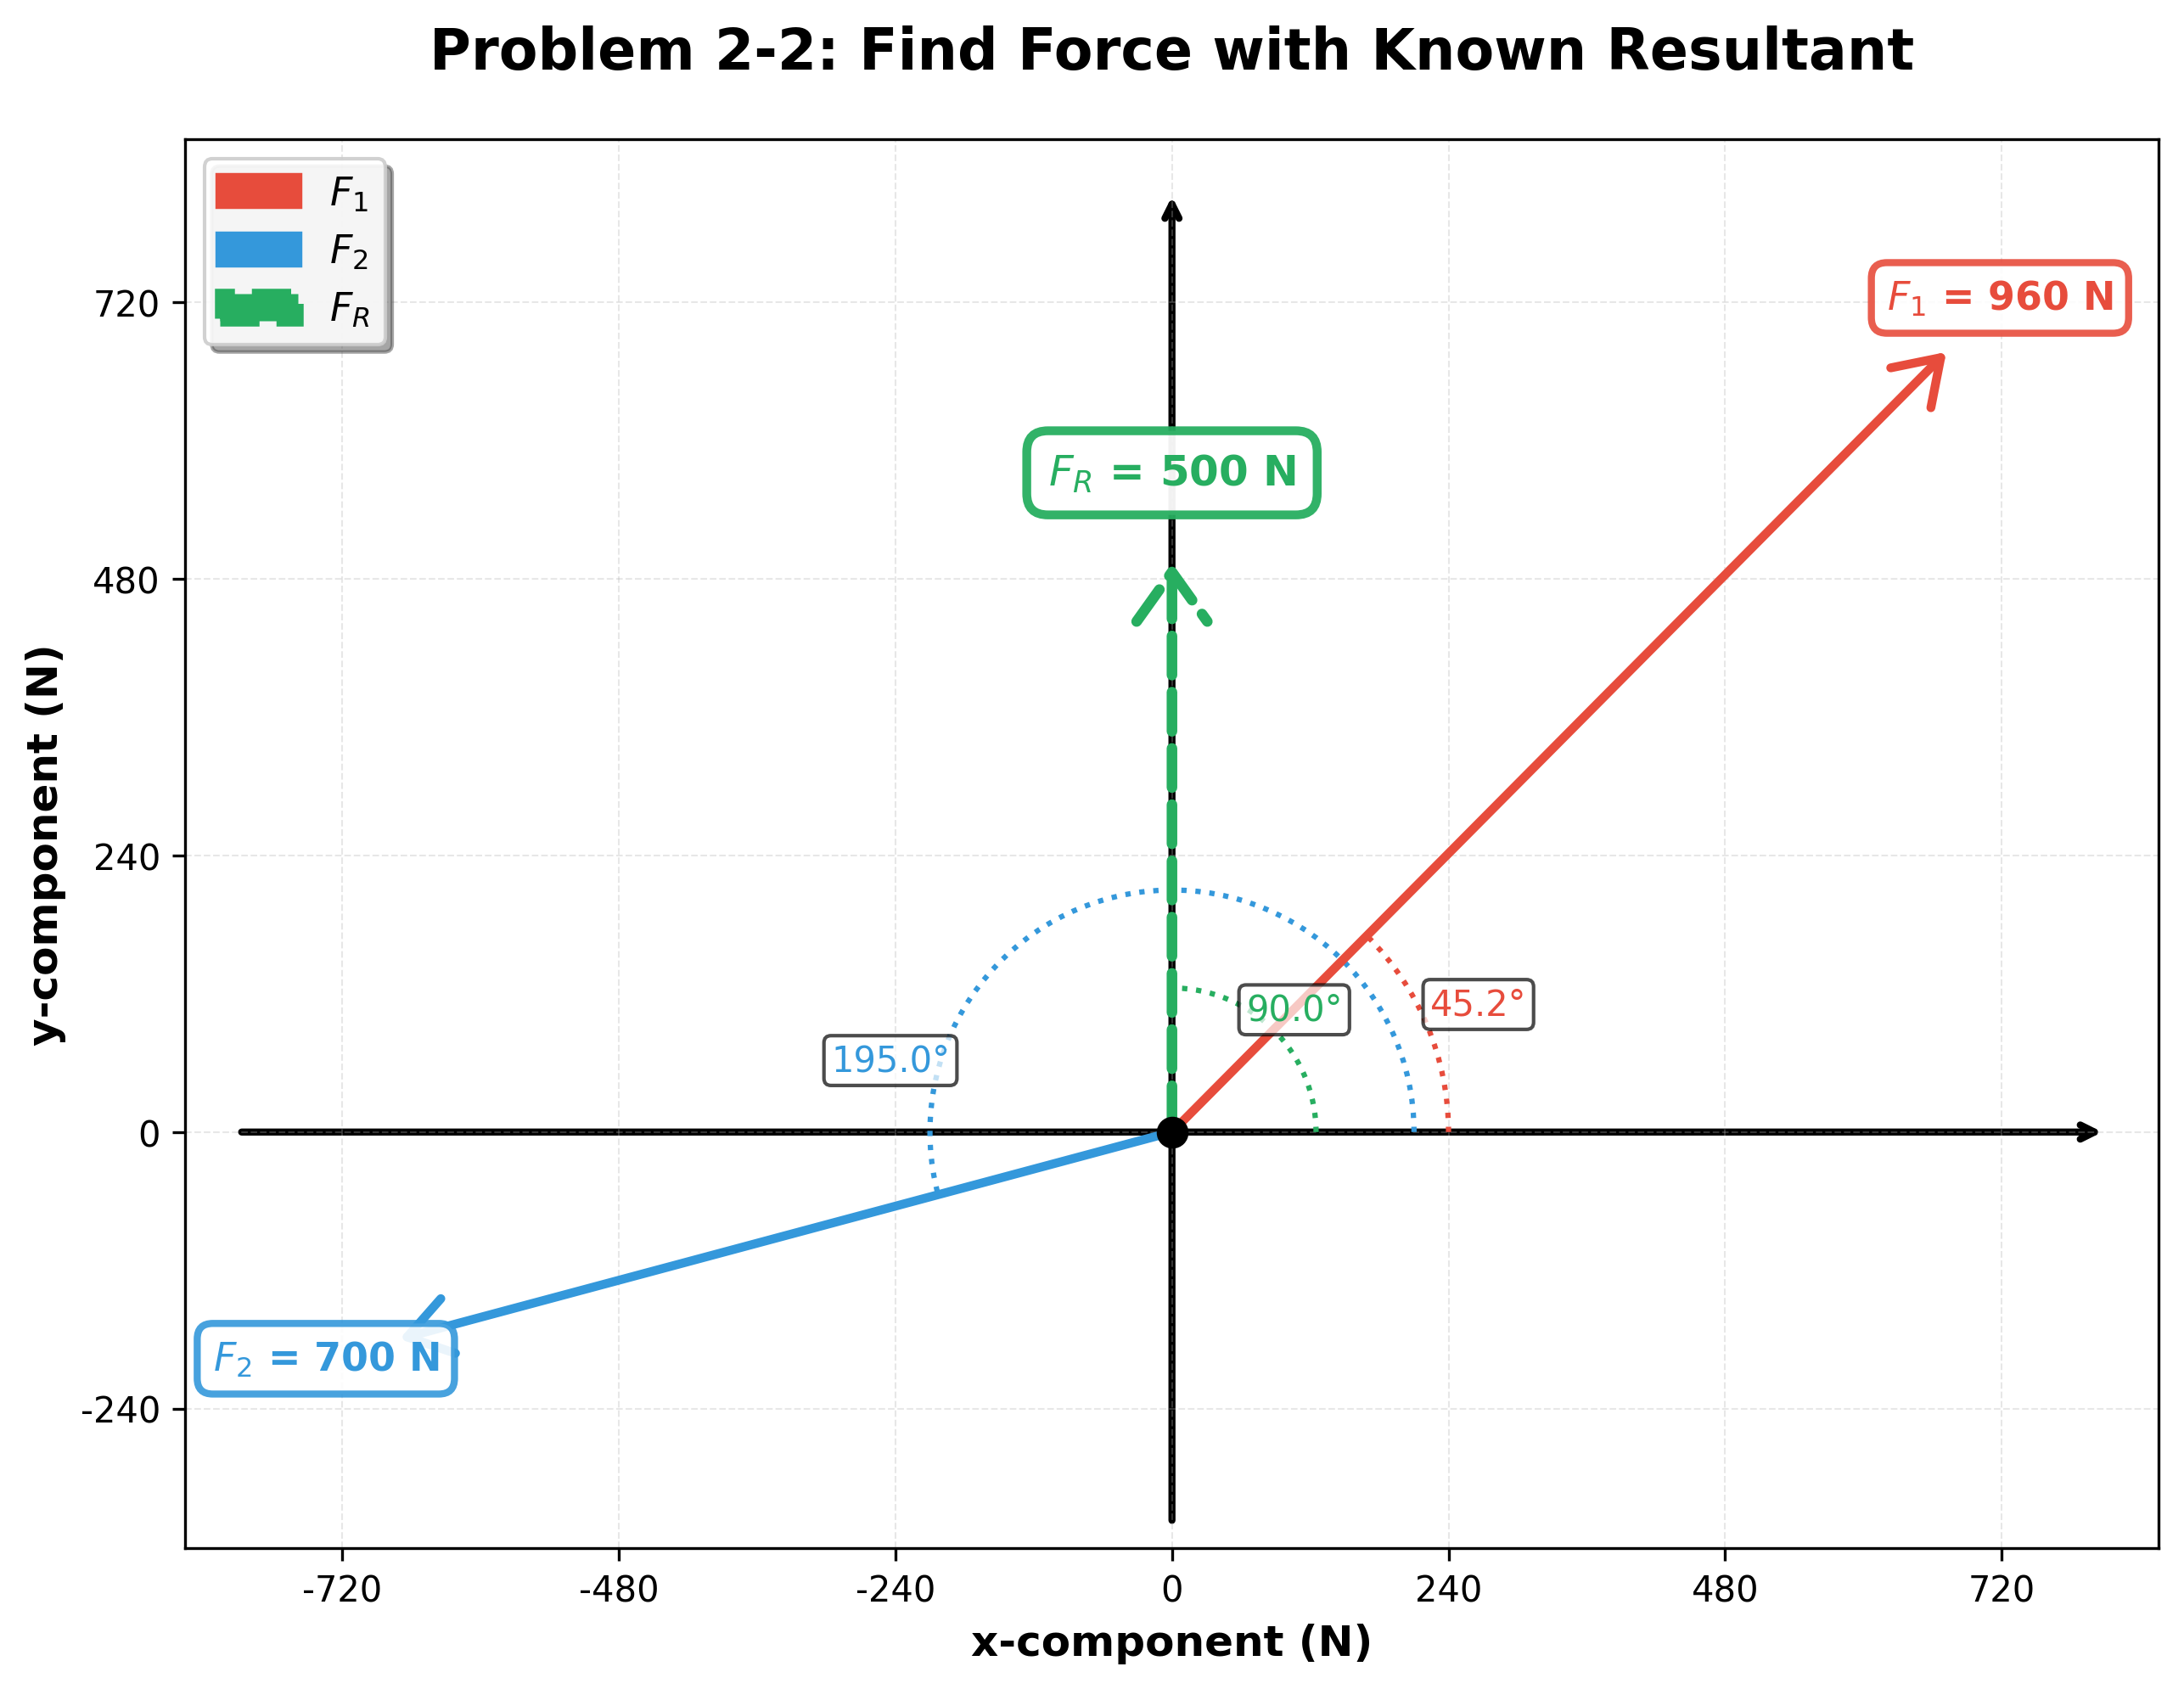
\includegraphics[width=0.7\textwidth]{Problem_2-2_Find_Force_with_Known_Resultant_diagram.png}
\end{center}

\begin{center}
\textit{Figure: Vector diagram showing all forces and their orientations}
\end{center}


\clearpage

\section*{Disclaimer}
\addcontentsline{toc}{section}{Disclaimer}

\begin{center}
\rule{\textwidth}{0.4pt}
\end{center}

\noindent\textbf{IMPORTANT NOTICE:}

\noindent While every effort has been made to ensure the accuracy and reliability of the calculations provided, we do not guarantee that the information is complete, up-to-date, or suitable for any specific purpose. Users must independently verify the results and assume full responsibility for any decisions or actions taken based on its output. Use of this calculator is entirely at your own risk, and we expressly disclaim any liability for errors or omissions in the information provided.

\vspace{1em}

\noindent\textbf{Report Details:}
\begin{itemize}
\item \textbf{Generated Date:} October 13, 2025
\item \textbf{Generated Using:} Qnty Library
\item \textbf{Version:} Beta (Independent verification required for production use)
\end{itemize}

\vspace{2em}

\noindent\textbf{Professional Review and Approval:}

\vspace{1em}

\begin{longtable}{|p{3cm}|p{4cm}|p{4cm}|p{2.5cm}|}
\hline
\textbf{Role} & \textbf{Name} & \textbf{Signature} & \textbf{Date} \\
\hline
\hline
Calculated By & \rule{0pt}{1.5cm} & & \\
\hline
Reviewed By & \rule{0pt}{1.5cm} & & \\
\hline
Approved By & \rule{0pt}{1.5cm} & & \\
\hline
\end{longtable}

\vspace{1em}

\begin{center}
\rule{\textwidth}{0.4pt}
\vspace{0.5em}
\textit{Report generated using Qnty Library}
\vspace{0.5em}
{\footnotesize For questions or support, please refer to the Qnty documentation}
\end{center}

\end{document}